% Created 2021-11-02 火 08:55
% Intended LaTeX compiler: pdflatex
\documentclass[dvipdfmx,11pat]{jarticle}
\usepackage[utf8]{inputenc}
\usepackage[T1]{fontenc}
\usepackage{graphicx}
\usepackage{grffile}
\usepackage{longtable}
\usepackage{wrapfig}
\usepackage{rotating}
\usepackage[normalem]{ulem}
\usepackage{amsmath}
\usepackage{textcomp}
\usepackage{amssymb}
\usepackage{capt-of}
\usepackage{hyperref}
\setlength{\textwidth}{18cm}
\setlength{\oddsidemargin}{-1cm}
\setlength{\evensidemargin}{-1cm}
\setlength{\topmargin}{-2cm}
\setlength{\textheight}{26cm}
\author{suzuki@iwate-u.ac.jp suzuki@iwate-u.ac.jp 鈴木正幸,岩手大学・非常勤講師}
\date{\today}
\title{数理情報科学特論 コンピュータと数式処理}
\begin{document}

\maketitle
\begin{center}
\large{\tt URL: https://github.com/masayuki054/comp\_and\_cal}
\end{center}

\section*{デジタル技術と協調しよう}
\label{sec:org094082a}

コンピュータとインターネットと上手に付き合って,

上手に,知り,考え,記憶し,検索し,思い出せるようにしよう。

知的作業を,外化して,共有しよう。

\begin{itemize}
\item \href{./org/digital\_tools.org}{思考とメモと文書のためのデジタル・ツール}

\begin{itemize}
\item 知識は構造
\item アウトライナー
\item マインドマップ
\item 文芸的プログラミング
\end{itemize}

\item \href{./org/web.org}{Web進化論}

\begin{itemize}
\item 集合知
\item 知識の構造化
\end{itemize}

\item \href{./org/comp\_thinking.org}{計算論的思考}

\begin{itemize}
\item 知的作業を見える化し,
\item 作業の流れを手続き化し,
\item コストを見積り,
\item 作業全体をデザインしよう
\end{itemize}

\item \href{./org/math-soft.org}{数学ソフトウェア}

\begin{itemize}
\item フリーソフトウェアを利用しよう
\item 数式処理システムと計算機代数アルゴリズム
\end{itemize}
\end{itemize}

\section*{規則と簡約化と検索のための計算機代数}
\label{sec:orgeac263d}

数学と検索と簡約のつながりについて,考えます。人は理論を考え,コン
ピュータに検索してもらいましょう。

多くの変数の高い次数の方程式の解法を,
線形代数の概念に翻訳し,
線形空間の概念と計算に帰着します。見通しと効率が良くなります。

\begin{itemize}
\item \href{./org/groebner.org}{グレブナー基底} 計算機代数アルゴリズムの紹介
\end{itemize}

\begin{figure}[htbp]
\centering
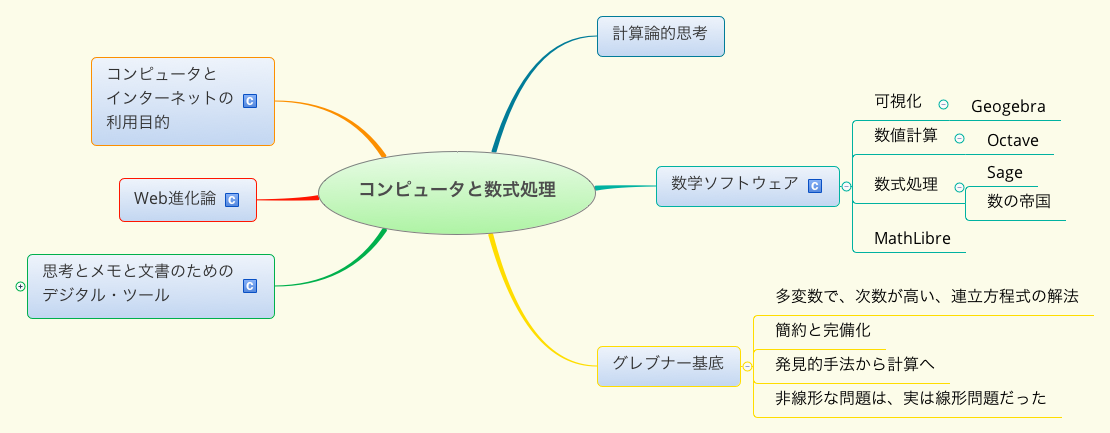
\includegraphics[width=18cm]{./map-images/01-computer_and_cal.png}
\caption{概要}
\end{figure}

\begin{figure}[htbp]
\centering
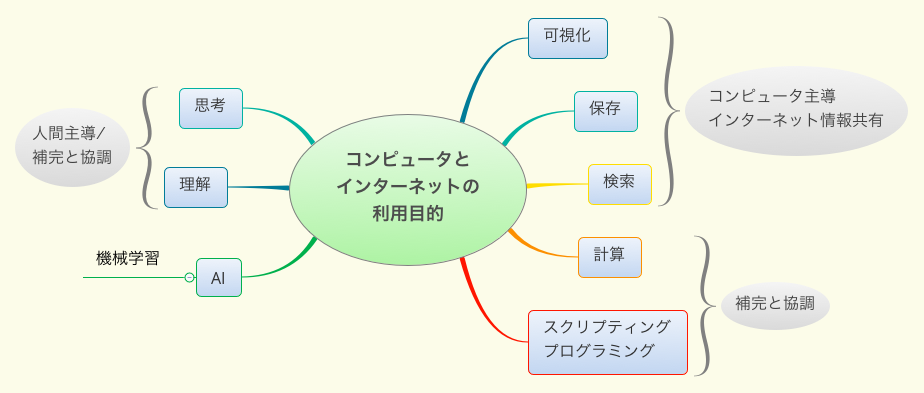
\includegraphics[width=18cm]{./map-images/03-how_to_use_computer_and_internet.png}
\caption{人とコンピュータとインターネット}
\end{figure}


\vspace{3cm}

\begin{figure}[htbp]
\centering
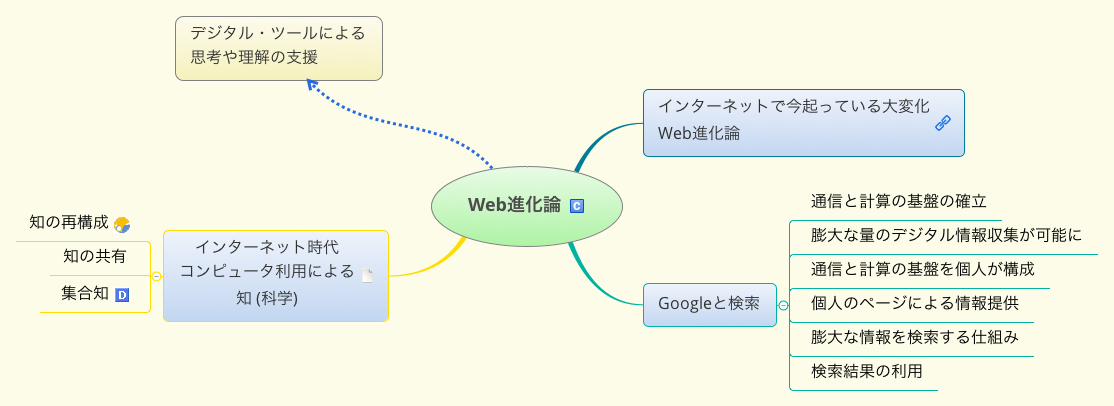
\includegraphics[width=18cm]{./map-images/04-Web_revolution.png}
\caption{インターネットが起している変革}
\end{figure}


\begin{figure}[htbp]
\centering
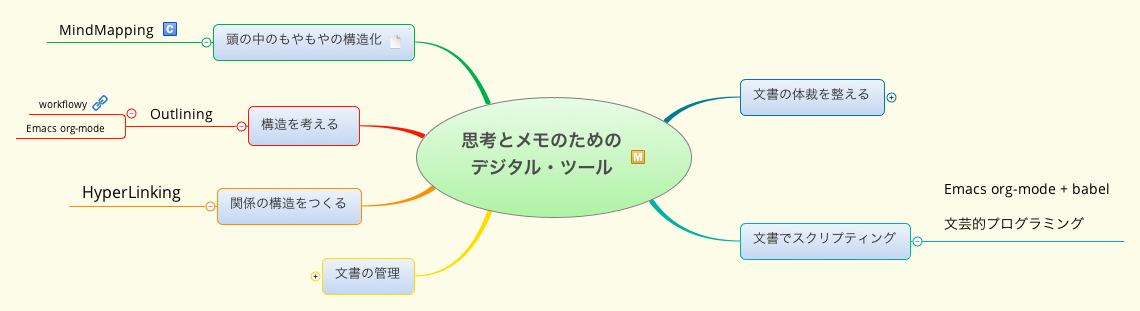
\includegraphics[width=18cm]{./map-images/05-digital_tools_for_thinking.png}
\caption{思考とメモと文書のためのデジタル・ツール}
\end{figure}


\section*{2020年度のまとめ}
\label{sec:org06c2f78}

\subsection*{{\bfseries\sffamily Doing} コンピュータと数式処理}
\label{sec:org1b128b4}
\begin{itemize}
\item 考えることをサポートするデジタルツールがある
\end{itemize}

\subsubsection*{考える,記憶する,こととは?}
\label{sec:orge43d54e}

\begin{itemize}
\item 思考の基本 抽象化と詳細化 , So What, Why so, MECE
\item 思考の記録 MECE, 構造化,GTD
\end{itemize}

\paragraph*{いろいろな思考法}
\label{sec:orgf8da2d0}
\begin{itemize}
\item 論理的思考
\item 批判的思考
\item 発想法
\item 水平思考
\item 計算論的思考
\end{itemize}

\paragraph*{知的思考の技術}
\label{sec:org2d8ae65}
\begin{itemize}
\item 思考の見える化
目的探索,観察,発想,分類,構造化,意志決定,表現
\end{itemize}

\subsubsection*{情報リテラシー}
\label{sec:org863fd49}

\begin{itemize}
\item 情報は 意味付けされたデータ
\end{itemize}

\paragraph*{知的情報リテラシーの技術}
\label{sec:orgba7ae4c}

\begin{itemize}
\item 情報の収集,加工,分析,蓄積,生成
\end{itemize}

\subsubsection*{コンピュータとインターネットによる思考の支援}
\label{sec:org1f54527}

\begin{itemize}
\item アウトライナー
\item マインドマップ
\end{itemize}

\subsection*{{\bfseries\sffamily Doing} メモと思考とdigital技術のまとめ}
\label{sec:org862b3fa}
\subsubsection*{理解を外化するためにコンピュータとインターネットを使おう}
\label{sec:orgc6ec9dd}

小さな理解のくりかえしを,構造的に記録する

\subsubsection*{内化しやすい外化}
\label{sec:org8d28200}

\paragraph*{理解しやすい外化}
\label{sec:org953eeab}

outline 

\paragraph*{イメージしやすい外化}
\label{sec:orgdfec351}

mindmap

\subsubsection*{外化の意味付}
\label{sec:org26ba242}

\begin{itemize}
\item 情報を外に出すことは二つの意味がある

\begin{itemize}
\item 内的情報を外部記憶に置くこと

こっちが外化, これがメモ

\item 自分の情報を他者が理解できる形にすること

第三者への情報 客観化,文書化
\end{itemize}
\end{itemize}

\paragraph*{理解と知識と外化}
\label{sec:org581ecea}

\begin{itemize}
\item 小さな理解と大きな理解,整合性の問題
\item 理解の再帰性
\end{itemize}

\subsubsection*{コンピュータとインターネットの意味}
\label{sec:org16ebd17}

\begin{itemize}
\item 情報を保存し共有すること
\item 検索できるようにすること
\item 人と計算機の共同作業の実現,互いに補完と拡張
\end{itemize}
\end{document}
